\documentclass[10pt,a4paper]{article}

\usepackage{fontspec}
\setmainfont{Times New Roman}
\usepackage[a4paper,margin=1.55cm]{geometry}
\usepackage{graphicx}
\usepackage{array}
\usepackage{tabularx}
\usepackage{booktabs}
\usepackage{enumitem}
\usepackage{xcolor}
\usepackage{titlesec}
\usepackage{caption}
\usepackage{hyperref}

\hypersetup{colorlinks=true, linkcolor=black, urlcolor=blue}
\setlength{\parindent}{0pt}
\setlength{\parskip}{2pt}
\renewcommand{\arraystretch}{1.12}
\setlist[itemize]{leftmargin=*, topsep=1pt, itemsep=1pt, parsep=0pt}
\setlist[enumerate]{leftmargin=*, topsep=1pt, itemsep=1pt, parsep=0pt}
\titlespacing*{\section}{0pt}{5pt}{3pt}
\titlespacing*{\subsection}{0pt}{4pt}{2pt}
\titleformat{\section}{\large\bfseries}{\thesection.}{0.45em}{}
\titleformat{\subsection}{\large\bfseries\color{blue!70!black}}{\thesubsection.}{0.45em}{}
\captionsetup{font=small, skip=2pt}
\newcolumntype{Y}{>{\raggedright\arraybackslash}X}
\emergencystretch=3em

\begin{document}
\pagenumbering{arabic}

\begin{center}
{\Large\bfseries Báo cáo bài tập lớn: Hệ thống đấu giá trực tuyến AuctionUET}\\[-1pt]
{\normalsize Môn Lập trình Nâng cao -- Trường Đại học Công nghệ, ĐHQGHN}\\[-1pt]
{\small Giảng viên: Phạm Bảo Phúc, Trần Ngọc Trúc Linh \quad | \quad Công nghệ: Java 21, Maven, JavaFX, Socket JSON}
\end{center}
\vspace{-4pt}

\section{Mục tiêu và phạm vi thực hiện}
AuctionUET được xây dựng nhằm mô phỏng một nền tảng đấu giá trực tuyến kiểu eBay Auctions: người bán đăng sản phẩm, người mua cạnh tranh giá trong một khoảng thời gian, hệ thống tự xác định người thắng và xử lý thanh toán. Phạm vi triển khai gồm ứng dụng JavaFX cho người dùng, server socket đa luồng, giao thức JSON dùng chung, lưu trữ JSON, kiểm thử JUnit và CI cơ bản.

Hệ thống tập trung vào các yêu cầu trong đề bài: quản lý người dùng theo vai trò Bidder/Seller/Admin, quản lý sản phẩm và phiên đấu giá, đặt giá hợp lệ, kết thúc phiên tự động, xử lý lỗi, giao diện đồ họa, realtime update, an toàn khi nhiều người đặt giá đồng thời. Nhóm cũng triển khai các phần nâng cao: ví điện tử và đặt cọc 10\%, auto-bidding, anti-sniping, biểu đồ giá realtime, dashboard quản trị và voice bidding qua Gemini.

\section{Kiến trúc tổng thể}
\begin{figure}[!ht]
    \centering
    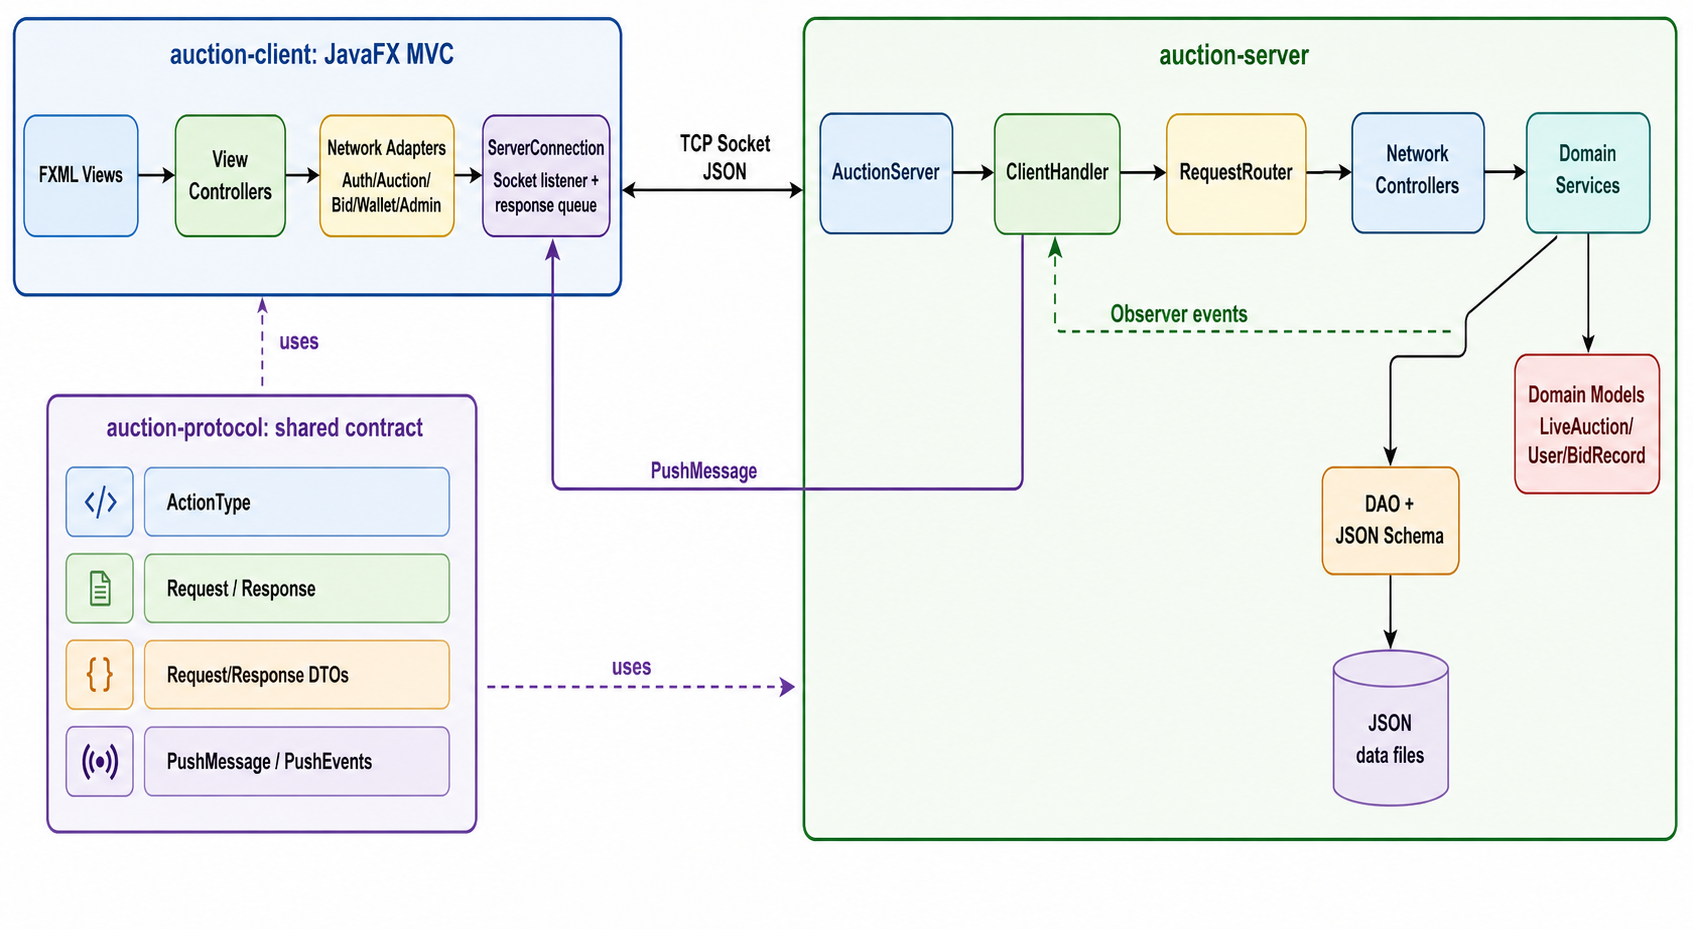
\includegraphics[width=\linewidth]{images/system_architecture.png}
    \caption{Kiến trúc Client--Server của AuctionUET.}
\end{figure}
\vspace{-6pt}

\begin{itemize}
    \item \textbf{Client JavaFX/MVC}: các màn hình FXML và controller nằm trong \texttt{auction-client}; controller chỉ điều phối UI, gọi các adapter mạng như \texttt{AuthClient}, \texttt{AuctionClient}, \texttt{BidClient}, \texttt{WalletClient}. Các lệnh mạng chạy ở background thread và cập nhật UI qua \texttt{Platform.runLater}.
    \item \textbf{Protocol contract-first}: module \texttt{auction-protocol} là nguồn sự thật chung cho \texttt{ActionType}, \texttt{Request}, \texttt{Response}, \texttt{PushMessage}, DTO request/response và enum nghiệp vụ. Cách này tránh tạo DTO lệch nhau giữa client và server.
    \item \textbf{Server phân tầng}: socket được xử lý bởi \texttt{AuctionServer}/\texttt{ClientHandler}; \texttt{RequestRouter} định tuyến tới controller; controller xác thực token/quyền rồi gọi service; service chứa nghiệp vụ và ghi qua DAO/schema JSON.
    \item \textbf{Realtime push}: client subscribe vào phiên; \texttt{LiveAuction} phát sự kiện qua Observer; \texttt{AuctionManager} chuyển tiếp tới các \texttt{ClientHandler}; server gửi \texttt{PushMessage} type \texttt{PUSH}; \texttt{ServerConnection} tách push khỏi response thường.
\end{itemize}

\section{Chức năng đạt được theo barem và bằng chứng}

\subsection*{Thiết kế lớp và cây kế thừa}
{\scriptsize
\setlength{\tabcolsep}{3pt}
\noindent
\begin{tabularx}{\linewidth}{>{\raggedright\arraybackslash\bfseries}p{0.20\linewidth} p{0.13\linewidth} Y Y}
\toprule
Mốc barem & Tự chấm điểm & Hướng giải quyết và lý do lựa chọn & Bằng chứng từ triển khai \\
\midrule
Các lớp chính: \texttt{User}, \texttt{Bidder/Seller/Admin}, \texttt{Item}, \texttt{Auction}, \texttt{BidTransaction} & 0.5 / 0.5 & Tách runtime domain và persistence schema: user runtime phục vụ phân quyền; sản phẩm/phiên/bid/giao dịch lưu bằng schema JSON. Cách này tránh đưa mật khẩu/hash vào domain trả về client. & \texttt{User}, \texttt{Bidder}, \texttt{Seller}, \texttt{Admin}; \texttt{ItemSchema}/\texttt{ItemDTO}; \texttt{AuctionSchema}/\texttt{AuctionDTO}; \texttt{BidRecord}/\texttt{BidSchema}; \texttt{TransactionSchema}/\texttt{TransactionDTO}. \\
\addlinespace
OOP: Encapsulation, Inheritance, Polymorphism, Abstraction & 1 / 1 & Dùng abstract class cho vai trò chung, override quyền theo từng role, field private/final và getter để bảo vệ state; \texttt{LiveAuction} đóng gói toàn bộ trạng thái phiên đang chạy. & \texttt{User} có abstract \texttt{hasPermission} và \texttt{getDisplayInfo}; \texttt{Bidder/Seller/Admin} override bằng \texttt{switch}; \texttt{LiveAuction} giữ \texttt{currentHighestBid}, \texttt{currentWinnerId}, \texttt{bidHistory} private. \\
\addlinespace
Design pattern phù hợp & 1 / 1 & Chọn pattern theo đúng bài toán: Singleton cho manager toàn cục, Observer cho push realtime, DAO cho JSON persistence, MVC cho UI/server, Factory cho Gson adapter. & \texttt{AuctionManager}, \texttt{DataManager}, \texttt{SessionManager}; \texttt{AuctionObserver}; \texttt{UserDAO}/\texttt{AuctionDAO}/\texttt{BidDAO}; \texttt{GsonFactory}; FXML/controller ở client và controller/service/DAO ở server. \\
\bottomrule
\end{tabularx}\par}

\subsection*{Chức năng chính}
{\scriptsize
\setlength{\tabcolsep}{3pt}
\noindent
\begin{tabularx}{\linewidth}{>{\raggedright\arraybackslash\bfseries}p{0.20\linewidth} p{0.13\linewidth} Y Y}
\toprule
Mốc barem & Tự chấm điểm & Hướng giải quyết và lý do lựa chọn & Bằng chứng từ triển khai \\
\midrule
Quản lý người dùng, sản phẩm & 1 / 1 & Người dùng đăng ký/đăng nhập/profile phân quyền theo vai trò; Seller quản lý sản phẩm; Admin phê duyệt/khóa tài khoản. Đặt nghiệp vụ trong service để controller mỏng. & \texttt{LOGIN}, \texttt{REGISTER}, \texttt{GET\_PROFILE}; \texttt{CREATE\_ITEM}, \texttt{GET\_MY\_ITEMS}, \texttt{DELETE\_ITEM}; \texttt{AuthService}, \texttt{UserService}, \texttt{ItemService}, \texttt{AdminService}; màn \texttt{Login/Register/MyItems/AdminItems}. \\
\addlinespace
Chức năng đấu giá & 1 / 1 & Server quyết định giá hợp lệ, người dẫn đầu, lịch sử bid và thanh toán; client chỉ gửi request. Cách này chống sửa giá từ UI và giữ dữ liệu nhất quán. & \texttt{CREATE\_AUCTION}, \texttt{START\_AUCTION}, \texttt{PLACE\_BID}, \texttt{GET\_BID\_HISTORY}, \texttt{PAY\_AUCTION}; \texttt{AuctionService}; \texttt{BidService.placeBid}; \texttt{LiveAuction.placeBid}; \texttt{BidDAO.save}. \\
\addlinespace
Xử lý lỗi và ngoại lệ & 1 / 1 & Validate DTO ở protocol và service; lỗi nghiệp vụ ném exception rõ nghĩa rồi chuyển về \texttt{Response.error}. Cách này giữ thông báo thống nhất và không lộ stack trace/sensitive data. & \texttt{ValidatableDTO}; \texttt{Request.fromDto}/\texttt{getDataAs}; \texttt{InvalidBidException}, \texttt{AuctionClosedException}, \texttt{InsufficientBalanceException}; \texttt{GlobalExceptionHandler}; test có case JSON lỗi/token lỗi/quyền lỗi. \\
\bottomrule
\end{tabularx}\par}

\subsection*{Kỹ thuật quan trọng và concurrency}
{\scriptsize
\setlength{\tabcolsep}{3pt}
\noindent
\begin{tabularx}{\linewidth}{>{\raggedright\arraybackslash\bfseries}p{0.20\linewidth} p{0.13\linewidth} Y Y}
\toprule
Mốc barem & Tự chấm điểm & Hướng giải quyết và lý do lựa chọn & Bằng chứng từ triển khai \\
\midrule
Đấu giá đồng thời an toàn & 1 / 1 & Giải quyết race condition và lost update: Dùng khóa riêng lẻ từng phiên đấu giá qua \texttt{ReentrantLock} tại \texttt{LiveAuction} để thu hẹp phạm vi lock. Gói kiểm tra nghiệp vụ và trừ tiền cọc ví điện tử trong các phương thức \texttt{synchronized} tại \texttt{WalletService} và \texttt{BidService}. Sử dụng các cấu trúc dữ liệu thread-safe \texttt{ConcurrentHashMap} và \texttt{CopyOnWriteArrayList} cho token và danh sách observer. & \texttt{BidService.placeBid}/\texttt{setAutoBid} synchronized; \texttt{WalletService} synchronized; \texttt{LiveAuction} dùng \texttt{ReentrantLock}; state dùng \texttt{ConcurrentHashMap}, \texttt{CopyOnWriteArrayList}; scheduler quản lý start/end. \\
\addlinespace
Realtime update qua Observer/Socket & 0.5 / 0.5 & Hiện thực Observer Pattern đa tầng: \texttt{LiveAuction} (Subject) gọi \texttt{notifyObservers} đẩy qua Socket dòng tin JSON đơn giản (\texttt{PushMessage} type \texttt{PUSH}). Client dùng luồng nền riêng (\texttt{daemon thread} của \texttt{ServerConnection}) đọc socket, đưa phản hồi thường vào \texttt{BlockingQueue} và chuyển trực tiếp tin push qua UI bằng \texttt{Platform.runLater}. & \texttt{SUBSCRIBE}/\texttt{UNSUBSCRIBE}; \texttt{PushActionType}, \texttt{PushEvents}, \texttt{PushMessage}; \texttt{ClientHandler.sendPush}; \texttt{ServerConnection} tách type \texttt{PUSH}; \texttt{BiddingController.onPushMessage}. \\
\bottomrule
\end{tabularx}\par}

\subsection*{Tích hợp, kiến trúc và chất lượng mã}
{\scriptsize
\setlength{\tabcolsep}{3pt}
\noindent
\begin{tabularx}{\linewidth}{>{\raggedright\arraybackslash\bfseries}p{0.20\linewidth} p{0.13\linewidth} Y Y}
\toprule
Mốc barem & Tự chấm điểm & Hướng giải quyết và lý do lựa chọn & Bằng chứng từ triển khai \\
\midrule
Kiến trúc Client--Server rõ ràng & 0.5 / 0.5 & Dùng TCP socket JSON, client không truy cập dữ liệu trực tiếp; mọi nghiệp vụ và persistence nằm ở server. & \texttt{AuctionServer}, \texttt{ClientHandler}, \texttt{RequestRouter}; \texttt{ServerConnection}; \texttt{MessageSerializer}; dữ liệu JSON trong \texttt{auction-server/data}. \\
\addlinespace
MVC: JavaFX+FXML, Controller--Model--DAO server & 0.5 / 0.5 & Client tách FXML view, controller và network adapter; server tách controller nhận request, service xử lý nghiệp vụ, DAO lưu dữ liệu. & 22 FXML trong \texttt{auction-client}; 22 controller view; server có \texttt{AuthController}, \texttt{BidController}, \texttt{AuctionController}; service/DAO/schema tương ứng. \\
\addlinespace
Maven/Gradle, convention, mã sạch & 0.5 / 0.5 & Maven multi-module giúp build contract trước rồi server/client dùng chung; package chia theo layer để tránh DTO/protocol trùng lặp. & Parent \texttt{pom.xml} khai báo 3 module; Java 21; dependency quản lý Gson, SLF4J, Logback, JUnit; source chia \texttt{protocol}, \texttt{network}, \texttt{domain}, \texttt{persistence}. \\
\addlinespace
Unit Test JUnit cho logic quan trọng & 0.5 / 0.5 & Test tập trung vào service, DAO, auth, auction flow, wallet và integration socket vì đây là các điểm dễ lỗi nghiệp vụ. & Repo có 29 file test Java; chạy cục bộ \texttt{mvn test --batch-mode} pass 148 test, 0 failure/error/skipped; ví dụ \texttt{AuctionServiceTest}, \texttt{WalletServiceTest}, \texttt{AuthIntegrationTest}. \\
\addlinespace
CI/CD cơ bản & 0.5 / 0.5 & GitHub Actions tự chạy test khi pull request vào \texttt{main}/\texttt{develop}, giảm rủi ro merge code lỗi. & \texttt{.github/workflows/ci.yml}: checkout, setup JDK 21 Temurin, cache Maven, chạy \texttt{mvn test --batch-mode}. \\
\bottomrule
\end{tabularx}\par}

\subsection*{Chức năng nâng cao}
{\scriptsize
\setlength{\tabcolsep}{3pt}
\noindent
\begin{tabularx}{\linewidth}{>{\raggedright\arraybackslash\bfseries}p{0.20\linewidth} p{0.13\linewidth} Y Y}
\toprule
Mốc barem & Tự chấm điểm & Hướng giải quyết và lý do lựa chọn & Bằng chứng từ triển khai \\
\midrule
Auto-Bidding với maxBid, increment & 0.5 / 0.5 & Người dùng đặt trần và bước giá qua \texttt{AutoBidConfig}. Chỉ người đang dẫn đầu mới được kích hoạt Auto-Bid nhằm loại bỏ hoàn toàn bidding wars. Khi leader cũ bị vượt mặt, sinh \texttt{PendingAutoBid} có sequenceId. Luồng chạy nền của server sẽ gọi \texttt{resolvePendingAutoBid} dưới khóa \texttt{ReentrantLock} để tự động nâng giá đè lên \texttt{currentHighest + increment} (không vượt \texttt{maxBid}). & \texttt{SetAutoBidRequestDTO}; \texttt{AutoBidConfig}; \texttt{LiveAuction.pendingAutoBid}; \texttt{resolvePendingAutoBid}; \texttt{BidService.schedulePendingAutoBidResponse}; \texttt{CHECK\_AUTO\_BID}. \\
\addlinespace
Anti-sniping khi bid cuối & 0.5 / 0.5 & Nếu có bid trong cửa sổ \texttt{antiSnipingWindowSeconds} trước khi hết giờ, tự động cộng thêm \texttt{antiSnipingExtensionSeconds} vào \texttt{endTime} của \texttt{LiveAuction}. Server phát sự kiện push \texttt{AUCTION\_EXTENDED}, đồng thời hủy bỏ task kết thúc cũ và lập lịch lại một kết thúc mới thông qua \texttt{ScheduledExecutorService.schedule}. & \texttt{LiveAuction.extendIfSniping}; \texttt{antiSnipingWindowSeconds}; \texttt{antiSnipingExtensionSeconds}; push \texttt{AUCTION\_EXTENDED}; \texttt{AuctionManager.extendAuction} schedule lại end task. \\
\addlinespace
Bid History Visualization realtime & 0.5 / 0.5 & Vẽ biểu đồ giá động dạng \texttt{LineChart} của JavaFX. Khi bắt được sự kiện push \texttt{BID\_UPDATE} từ server ở background thread, Client bọc lời gọi \texttt{appendBidPricePoint} bên trong \texttt{Platform.runLater} để cập nhật mượt mà các điểm dữ liệu mới (\texttt{XYChart.Data}) lên biểu đồ theo thời gian thực mà không cần tải lại trang. & \texttt{LineChart<Number, Number>} trong \texttt{BiddingController}; \texttt{appendBidPricePoint}; \texttt{loadBidHistory}; \texttt{onPushMessage} xử lý \texttt{BID\_UPDATE}. \\
\addlinespace
Tính năng sáng tạo khác & 0.5 / 0.5 & Ví điện tử đóng băng cọc 10\% (\texttt{freezeDeposit}), lưu chi tiết qua \texttt{TransactionSchema} phục vụ kiểm toán tài chính. Giám sát hệ thống qua \texttt{SystemMonitorService}. Tích hợp Voice Bidding: ghi âm từ mic, truyền raw audio bất đồng bộ tới \texttt{Google Gemini API} (\texttt{gemini-3.5-flash} kết hợp system prompt) để nhận diện số tiền tiếng Việt thành số thực tự động. & \texttt{WalletService.holdAuctionDeposit}; \texttt{TransactionService}; \texttt{AdminFinancialController}; \texttt{SystemMonitorService}; \texttt{GeminiVoiceServiceClient}; \texttt{VoiceConfigView.fxml}. \\
\bottomrule
\end{tabularx}\par}

\vspace{2pt}
\section{Phân chia công việc}
\small
\begin{tabularx}{\linewidth}{p{0.18\linewidth} p{0.13\linewidth} p{0.19\linewidth} Y}
\toprule
Thành viên & MSSV & Vai trò & Đóng góp chính \\
\midrule
Tạ Hữu Cường & 25020053 & Team Leader, Core Architect & Phát triển tầng service Auction/Wallet/Bid, refactor sản phẩm sang \texttt{ItemSchema} phẳng, tích hợp Gemini Voice Input/Bidding, kiểm soát concurrency và luồng thanh toán. \\
Ngô Duy Anh & 25020015 & Lead Backend, Quality & Thiết kế OOP domain model, hệ thống Admin, integration tests và tài liệu viva/kiểm thử. \\
Nguyễn Cao Công & 25020046 & Frontend Lead, Client Dev & Phát triển 22 giao diện JavaFX FXML/CSS, quản lý network connection phía client, Theme Manager và xử lý UI bằng \texttt{Platform.runLater}. \\
Đào Đình Khánh & 25020211 & Network, DevOps Lead & Thiết kế protocol \texttt{Request/Response/Push}, socket server và request routing, auto-bidding bảo vệ người dẫn đầu (Pending State), thiết lập GitHub Actions CI. \\
\bottomrule
\end{tabularx}
\normalsize

\section{Kết luận}
AuctionUET đáp ứng các yêu cầu bắt buộc của đề bài và bổ sung các chức năng nâng cao có bằng chứng trực tiếp trong mã nguồn. Cách triển khai ưu tiên contract-first, phân tầng rõ ràng và xử lý đồng thời ở server, giúp hệ thống vận hành nhất quán khi nhiều client cùng tham gia một phiên đấu giá.

\end{document}
